\section{Extracting a long prime prefix}\label{sec:extraction}

Our first task is to represent almost every totient by a long prime
prefix and a bounded arithmetic tail.  The exceptional set must be
small in a stronger sense: outside it, \emph{every} preimage must have
the required form.  Later we shall count distinct prefix--tail tuples,
and remove tuples that fail the conditions needed to compare two
representations.

Throughout this section \(H\) is a sufficiently large fixed integer,
\(P=\lfloor\log\log H\rfloor\), and
\begin{equation}\label{eq:cuts}
 R=m-H,\qquad L=m-P.
\end{equation}
We first let \(x\to\infty\), and then let \(H\to\infty\).
Write \(h_i=m-i\) and
\[
 \alpha=\frac{B\rho^m}{m},\qquad
 b_i=\alpha h_i\rho^{-h_i},\qquad
 \widetilde b_i=\alpha_\theta h_i\rho^{-h_i},\qquad
 \xi_i=1+10^{-4}\e^{-h_i/40}.
\]
In particular \(b_0=B\).  The definitions in
\eqref{eq:scales} give
\begin{equation}\label{eq:alpha-comparison}
 \frac{\alpha}{\alpha_\theta}
 =\frac{\log B}{\lambda m}
 =1+\frac{\lambda\theta+\log\log B}{\lambda m}
 =1+O\left(\frac{\log m}{m}\right).
\end{equation}
Thus \(\alpha\) and \(\alpha_\theta\) stay in a fixed compact
subinterval of \((0,\infty)\), uniformly in the phase.
We shall only need the coarse bounds
\begin{equation}\label{eq:rho-bounds}
 0.54<\rho<0.545,
\end{equation}
which follow from the numerical value recorded in
\cite[(1.4)]{FordTotients2013}.  They imply
\(\lambda<1\), \(18<30\lambda<20\), and \(1.1\rho<0.6\).
Together with \eqref{eq:alpha-comparison}, these inequalities
justify the fixed constants \(0.61\) and \(0.62\) used below.
We use
\[
 K_H=\exp(CP\rho^{-P})=H^{o(1)},
\]
where the absolute constant \(C\) may be enlarged from one upper bound
to the next.  The last equality follows from
\(\lambda=\log(1/\rho)<1\).
The notation \(\varepsilon_H\) denotes a positive quantity tending to
zero with \(H\), and \(o_{x;H}(1)\) denotes a quantity tending to zero
as \(x\to\infty\) for fixed \(H\).  All such estimates below are uniform
in the phase.

\subsection{Structure estimates from Ford}

Ford's order estimate and fundamental-simplex estimates give
\begin{equation}\label{eq:ford-scale}
 V(x)\asymp \frac{x}{\log x}G_m,
\end{equation}
and his recurrence estimate gives
\begin{equation}\label{eq:g-asymptotic}
 g_j=\gamma\rho^{-j}+O(1),\qquad g_j\asymp\rho^{-j}.
\end{equation}
See \cite[Theorem 1, Lemmas 3.4 and 3.7, and Corollary 3.5]
{FordTotients2013}.  Ford denotes our constant \(\gamma\) by
\(\lambda\).  In particular, for \(0\le j\le m\),
\begin{equation}\label{eq:G-uniform}
 \frac{G_j}{G_m}
 =\prod_{i=j+1}^m\frac{ig_i}{B}
 \le C^{m-j}\rho^{(m-j)(m-j-1)/2}\ll1.
\end{equation}

We shall use two quantitative structure results of Ford.
Order the prime factors of a preimage \(n\) with repetitions as
\(p_0\ge p_1\ge\cdots\).
For each fixed \(0<\eta\le1/8\), his Theorem 10, together with the
missing-prime exception in Theorem 16, implies
\begin{equation}\label{eq:ford-bands}
 \#\left\{v\le x:\begin{array}{l}
 v\in\mathcal V,\ \text{some preimage has}\\
 |\log_2p_i/b_i-1|>\eta\text{ for some }1\le i\le m-P
 \end{array}\right\}
 \ll_\eta V(x)\e^{-c_\eta P}.
\end{equation}
Here and below a missing indicated prime is a failure of the condition.
For completeness, the summation giving \eqref{eq:ford-bands} is short.
For \(i\le3\eta m\), Theorem 10(b) contributes at most
\(Cm\e^{-\eta m/13}V(x)\).  For \(i>3\eta m\), Theorem 10(a)
contributes at most
\[
 C V(x)\frac{i}{\eta m}
 \exp\left\{-\frac{\eta^2m(m-i)}{4i}\right\}
 \le \frac{CV(x)}{\eta}\e^{-\eta^2(m-i)/4}.
\]
Summing over \(m-i\ge P\) proves the assertion for sufficiently
large \(x\) when the indicated primes exist.  A missing \(p_L\) is
included in the \(O(V(x)\e^{-P^2/4})\) exceptional set of
Theorem 16, which is absorbed in the displayed bound.
The convention preceding Ford's Theorem 10 counts values
with \emph{some} failing preimage; hence the complement of this set
controls every preimage.

Ford's Theorem 16, with its parameter \(\Psi=P\), states that all but
\(O(V(x)\e^{-P^2/4})\) values have every preimage satisfying
\begin{equation}\label{eq:ford-simplex}
 \log_2p_L>2,\qquad
 \sum_{r=i+1}^L a_{r-i}u_r\le\xi_i u_i\quad(0\le i<L),
 \qquad u_0=B,\quad u_i=\log_2p_i\ (i\ge1).
\end{equation}
Its final adjacent-coordinate inequality has coefficient \(1\)
in place of \(a_1<1\); weakening that inequality gives
\eqref{eq:ford-simplex}.

Write \(\Omega(n,U,T)\) for the number of prime factors of \(n\)
belonging to \((U,T]\), counted with multiplicity, and put
\(\Omega(n)=\Omega(n,1,n)\), including \(\Omega(1)=0\).

\begin{definition}\label{def:normal}
For \(S\ge\e^\e\), a prime \(p\) is \(S\)-normal if
\[
 \Omega(p-1,1,S)\le2\log_2S
\]
and, for every \(S\le U<T\le p-1\),
\[
 \left|\Omega(p-1,U,T)-(\log_2T-\log_2U)\right|
 <\sqrt{\log_2S\,\log_2T}.
\]
\end{definition}
We use Definition 1 in the 2013 revision \cite{FordTotients2013}.
Its Lemma 2.6 gives, uniformly for \(z\ge3\),
\begin{equation}\label{eq:normal-primes}
 \#\{p\le z:p\text{ is not }S\text{-normal}\}
 \ll \frac{z}{\log z}(\log_2z)^5(\log S)^{-1/6}.
\end{equation}
The function \(\Omega\) in these statements counts prime factors with
multiplicity.

\subsection{Basic witnesses and the coverage target}

We now specify the representations that these structure estimates will
provide. The simplex notation records the inequalities on their prime
coordinates; the bounds on the last factor will make the arithmetic
tail finite for fixed \(H\).

For integers \(1\le j\le m\), \(u_0=B\), and \(\beta_i\ge1\) for \(0\le i<j\),
put \(\beta_j=1\) and define the simplex
\[
 S_j(\boldsymbol\beta)=
 \left\{(u_1,\ldots,u_j):
 s_i:=\beta_i u_i-\sum_{r=i+1}^j a_{r-i}u_r\ge0
 \quad(0\le i\le j)\right\}.
\]
The terminal inequality is \(u_j\ge0\).
For \(j=0\), the simplex consists of the empty tuple and has volume
\(G_0=1\).

\begin{definition}\label{def:basic}
A \emph{basic witness} is a choice of primes \(p_0,\ldots,p_L\)
and an integer \(a\ge1\) satisfying
\begin{equation}\label{eq:basic}
 \begin{gathered}
 p_0\ge x^{0.9},\qquad
 0.9\widetilde b_i\le\log_2p_i\le1.1\widetilde b_i
 \quad(1\le i\le L),\\
 (u_1,\ldots,u_L)\in S_L(\boldsymbol\xi),\qquad
 P^+(a)\le p_L,\qquad \log a\le\exp(2\widetilde b_L).
 \end{gathered}
\end{equation}
Here \(u_0=B\), and \(u_i=\log_2p_i\) for \(i\ge1\).
\end{definition}
For our parameter range the prime bands are disjoint and decreasing;
also \(p_0>p_1\).  Thus the displayed prime prefix is strictly
decreasing.  Repetitions of \(p_L\) inside \(a\) are allowed.

\begin{figure}[ht]
\centering
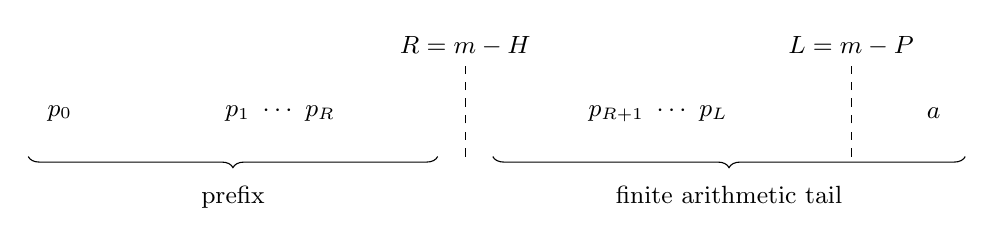
\begin{tikzpicture}[x=1cm,y=1cm,font=\small]
 \node at (0.4,0.45) {$p_0$};
 \node at (3.2,0.45) {$p_1\ \cdots\ p_R$};
 \node at (8,0.45) {$p_{R+1}\ \cdots\ p_L$};
 \node at (11.5,0.45) {$a$};
 \draw[dashed] (5.55,-0.1)--(5.55,1.05);
 \draw[dashed] (10.45,-0.1)--(10.45,1.05);
 \node[above] at (5.55,1.05) {$R=m-H$};
 \node[above] at (10.45,1.05) {$L=m-P$};
 \draw[decorate,decoration={brace,mirror,amplitude=4pt}]
       (0,-0.1)--(5.2,-0.1);
 \draw[decorate,decoration={brace,mirror,amplitude=4pt}]
       (5.9,-0.1)--(11.9,-0.1);
 \node[below] at (2.6,-0.35) {prefix};
 \node[below] at (8.9,-0.35) {finite arithmetic tail};
\end{tikzpicture}
\caption{The two cuts in a basic witness. We count $p_0$ by the prime
number theorem and approximate the $p_1,\ldots,p_R$ coordinates by volume.
The later primes and the smooth integer $a$ remain discrete.}
\label{fig:two-cuts}
\end{figure}

\begin{proposition}\label{prop:basic}
There is a set \(E_x\subseteq\mathcal V\cap[1,x]\) with
\[
 |E_x|\le\{\varepsilon_H+o_{x;H}(1)\}V(x)
\]
such that every preimage of every
\(v\in(\mathcal V\cap[1,x])\setminus E_x\) is
\(p_0\cdots p_La\) for a basic witness.  One may take
\[
 \varepsilon_H\ll
 \e^{-cP}+K_H\exp\{-\exp(cP\rho^{-P})\}.
\]
For every basic witness, putting \(w=p_{R+1}\cdots p_La\), we have
\begin{equation}\label{eq:cofactor-size}
 \begin{gathered}
 p_1\cdots p_La\le\exp((\log x)^{0.8}),\\
 \log w\le H\exp(0.62b_R)+\exp(2\widetilde b_L),
 \qquad w<p_R.
 \end{gathered}
\end{equation}
In particular \(w\) is bounded in terms of \(H\) alone, uniformly
in the phase.
\end{proposition}

We prove the proposition after the volume and smooth-cofactor estimates
below. Those estimates also prepare a second task: we shall retain the
shortened data \((p_0,\ldots,p_R,\varphi(w))\), then delete those
that fail the strict inequalities and normality conditions needed for
the collision argument. Coverage concerns \emph{values}; this later
deletion must count the distinct shortened tuples, including all tuples
that represent the same value.

\subsection{Simplex volume and concentration}
The coordinate scaling follows Ford's fundamental-simplex method
\cite[Lemma~3.2 and Corollary~3.3]{FordTotients2013}.
Our last adjacent coefficient is $a_1$ rather than $1$, so the exact
volume is slightly different from his; we derive it from the slacks
below. The recurrence estimate \eqref{eq:g-asymptotic} is Ford's
Lemma~3.7; his Remark~1 credits its streamlined proof to Lau's solution
of a recurrence problem \cite{FordLau2000}.

The next estimates turn sums over the allowed prime coordinates into
simplex volumes. We also bound the mass near a coordinate boundary or
a simplex face, so that removing these regions has a controlled cost.

\begin{lemma}\label{lem:simplex}
Let \(1\le j\le m\).  The true simplex \(S_j(\boldsymbol1)\) has volume \(G_j\).
Under its uniform volume measure the variables \(W_i=g_is_i/B\)
are uniform on \(\{W_i\ge0:\sum_{i=0}^jW_i=1\}\).
Moreover,
\[
 \operatorname{Vol}S_j(\boldsymbol\beta)
 \le G_j\prod_{r<j}\beta_r^{j-r}.
\]
Within \(S_j(\boldsymbol\beta)\), a specified slack \(s_t\) in an
interval of length \(D\) occupies at most a fraction \(jg_tD/B\)
of the volume.  A specified coordinate \(u_t\), \(1\le t\le j\),
in such an interval occupies at most \(jg_t\beta_tD/B\).
\end{lemma}

\begin{proof}
For the true simplex the triangular inversion is
\[
 u_i=\sum_{t=i}^j g_{t-i}s_t,\qquad
 B=\sum_{t=0}^j g_ts_t.
\]
The transformation from \(u_1,\ldots,u_j\) to \(s_1,\ldots,s_j\)
has determinant \(1\).  This proves the volume and distribution
statements.

Set \(K_i=\prod_{r<i}\beta_r\), \(K_0=1\).
The map \(u_i\mapsto u_i/K_i\) sends
\(S_j(\boldsymbol\beta)\) into \(S_j(\boldsymbol1)\), because
\(K_r\ge\beta_iK_i\) when \(r>i\).  Its inverse Jacobian is
\(\prod_{r<j}\beta_r^{j-r}\).

For the slice estimates, define
\(\gamma'_0=1\) and
\(\gamma'_t=\beta_t^{-1}\sum_{i<t}\gamma'_ia_{t-i}\).
Then \(0<\gamma'_t\le g_t\) and
\[
 \sum_{t=0}^j\gamma'_ts_t=\beta_0B.
\]
The marginal density of \(s_t\), under the uniform measure on this
simplex, is at most \(j\gamma'_t/(\beta_0B)\).
For the coordinate assertion, fix all other positive-index slacks.
The coordinate \(u_t\) is affine in \(s_t\) with slope \(1/\beta_t\).
Integrating first in this fiber and bounding by the full projection
volume gives the additional factor \(\beta_t\).
\end{proof}

The following concentration estimate will be used in Section~\ref{sec:limits}
to remove the prefix bands after replacing prime sums by volumes.
Write $z_+=\max\{z,0\}$.

\begin{lemma}\label{lem:concentration}
Fix \(\eta>0\).  There are constants \(C_\eta,c_\eta>0\) such that,
if \(Q\) is an integer with \(0\le Q<m\), \(j=m-Q\),
\(1\le i\le j\), and \(h_i\ge C_\eta(Q+1)\), then
uniform volume measure on \(S_j(\boldsymbol1)\) satisfies
\[
 \Pr(|u_i/b_i-1|>\eta)\le C_\eta\e^{-c_\eta h_i}.
\]
Also, for \(T\ge0\),
\[
 \Pr(u_j\ge T)=(1-g_jT/B)_+^j\le\e^{-jg_jT/B}.
\]
\end{lemma}

\begin{proof}
By \eqref{eq:g-asymptotic} and Lemma~\ref{lem:simplex},
\[
 \frac{u_i}{B\rho^i}
 =\sum_{t=i}^j(1+O(\rho^{t-i}))W_t.
\]
Represent \(W_t=E_t/\sum_{r=0}^jE_r\), where the \(E_t\) are
independent mean-one exponential variables.  The main numerator has
\(j-i+1=h_i-Q+1\) terms, and
\[
 \frac{(j-i+1)/(j+1)}{h_i/m}
 =1+O((Q+1)/h_i).
\]
Exponential moment bounds give exponentially small probabilities
for a fixed relative deviation of either the numerator or the
denominator.  The error numerator is bounded in absolute value by
\(C\sum_{r\ge0}\rho^rE_{i+r}\); this sum has a uniformly bounded
exponential moment, since
\(\prod_{r\ge0}(1-z\rho^r)^{-1}<\infty\) for \(0<z<1\).
Once \(h_i\ge C_\eta(Q+1)\), these three bounds give the first
assertion.  The second is the exact marginal tail of \(W_j\).
\end{proof}

\subsection{Prime boxes and smooth cofactors}
The use of reciprocal prime sums and enlarged coordinate boxes follows
Ford's Lemma~3.1 and the thickening arguments of his Section~3
\cite{FordTotients2013}. We record the quantitative bounds for our
simplexes, including the boundary errors needed for the tail unions.

We use unit boxes in the coordinates \(\log_2p_i\).
Mertens' theorem gives
\begin{equation}\label{eq:mertens-box}
 \sum_{b\le\log_2p<b+1}\frac1{p-1}=1+O(\e^{-b})
 \qquad(b\ge2).
\end{equation}
The replacement of \(1/p\) by \(1/(p-1)\) changes the sum by
\(O(\exp(-\exp b))\).  When the lower endpoints grow geometrically
backwards through the coordinates, multiplying
\eqref{eq:mertens-box} costs only a bounded factor; if their sum
of errors is small, it is the relative product error.

\begin{lemma}\label{lem:boxes}
Let \(0\le j\le L\).  Sum over primes \(p_1,\ldots,p_j\) whose
coordinates satisfy
\[
 0.9\widetilde b_i\le u_i\le1.1\widetilde b_i,\qquad
 (u_1,\ldots,u_j)\in S_j(\boldsymbol\xi).
\]
Then
\begin{equation}\label{eq:projected-mass}
 \sum_{p_1,\ldots,p_j}\prod_{i=1}^j\frac1{p_i-1}\ll G_m.
\end{equation}
Every unit box meeting this region lies in
\(S_j(\boldsymbol\beta)\), where, with a sufficiently large absolute
constant,
\begin{equation}\label{eq:box-enlargement}
 \beta_t=1+C\bigl(\e^{-h_t/40}+h_t^2\rho^{h_t}\bigr)
 \quad(0\le t<j),\qquad \beta_j=1.
\end{equation}
This enlargement has bounded volume cost.  Its coordinate scaling
factors through \(R\) differ from \(1\) by
\(O(\e^{-H/40}+H^2\rho^H)\).

There is also the following shell estimate in \(L\) coordinates.
Fix \(A>0\).  Among unit boxes meeting the displayed region, retain
those with a point satisfying, for some \(i\le R\), at least one of
these conditions:
\begin{enumerate}[label=(\roman*)]
\item \(i\ge1\) and \(u_i\) is within \(A\) of a coarse band endpoint;
\item the absolute value of
\(\xi_i u_i-\sum_{r=i+1}^L a_{r-i}u_r\) is at most \(Ah_i^2\);
\item \(\sum_{r=i+1}^L a_{r-i}u_r\ge(1-h_i^{-4})u_i\).
\end{enumerate}
The total volume of these boxes, and their total reciprocal-prime
weight, is
\begin{equation}\label{eq:boundary-mass}
 O_A(H^{-2}G_m).
\end{equation}
The same estimate holds when any subset of coordinates uses
reciprocal-prime measure and the others use Lebesgue measure.
For conditions (i)--(ii) alone, or for the region lost by replacing
the prefix coefficients \(\xi_i\), \(0\le i\le R\), with \(1\),
the stronger bound is
\[
 O_A\left(G_m\sum_{h\ge H}
       (h\e^{-h/40}+h^3\rho^h)\right).
\]
\end{lemma}

\begin{proof}
The band lower bounds are \(u_t\gg h_t\rho^{-h_t}\).
Changing each coordinate by at most \(1\) changes inequality \(t\)
by \(O(h_t^2)\).  These errors are absorbed by
\eqref{eq:box-enlargement}, including at \(t=0\), where \(u_0=B\)
is fixed.  The logarithm of its Jacobian upper bound is at most
\[
 C\sum_{h\ge P}h\bigl(\e^{-h/40}+h^2\rho^h\bigr)\ll1.
\]
Lemma~\ref{lem:simplex}, \eqref{eq:G-uniform}, and
\eqref{eq:mertens-box} prove \eqref{eq:projected-mass}.
The coordinate scaling factor is \(\prod_{t<i}\beta_t\), without
the Jacobian exponents; summing for \(h_t>h_i\ge H\) proves its
stated bound.

For the shells put \(h=h_i\).  Throughout a box meeting the bands,
\(u_i\ll b_i\).  Conditions (ii) and (iii), together with the unit
perturbations, put the enlarged slack in an interval starting at
zero of length at most
\[
 C_A\{b_i(h^{-4}+\e^{-h/40})+h^3\}.
\]
Here the \(h^3\) term includes
\(h^2\rho^hu_i=O(h^3)\).
Since \(Lg_i/B\ll\rho^h\), Lemma~\ref{lem:simplex} bounds the
relative volume by
\[
 C_A(h^{-3}+h\e^{-h/40}+h^3\rho^h).
\]
Condition (i), after expanding its interval by \(2\), costs only
\(O_A(\rho^h)\).  Sum these estimates over \(h\ge H\), and use
the bounded enlargement cost.  The prime-weight assertion follows
again from \eqref{eq:mertens-box}.
For the stronger assertion, omit \(h^{-4}\) from the slack interval.
Changing \(\xi_i\) to \(1\), for \(i\le R\), only removes points whose old slack is
between \(0\) and \((\xi_i-1)u_i\), which obey the same bound.
Finally every full unit box has uniformly bounded mass when an
arbitrary subset of its coordinates uses reciprocal-prime measure:
multiply the factors in \eqref{eq:mertens-box} for precisely that
subset.  This proves the mixed-measure assertion as well.
\end{proof}

\begin{lemma}\label{lem:smooth-tail}
Uniformly for \(Y\ge\exp(\exp2)\) and \(Z\ge0\),
\[
 \sum_{P^+(a)\le Y}\frac{a^{1/\log Y}}{\varphi(a)}\ll\log Y,
 \qquad
 \sum_{\substack{P^+(a)\le Y\\\log a>Z}}\frac1{\varphi(a)}
 \ll(\log Y)\exp(-Z/\log Y).
\]
In particular, with \(Y=\exp\exp(1.1\widetilde b_L)\),
\begin{equation}\label{eq:smooth-cost}
 \sum_{P^+(a)\le Y}\frac1{\varphi(a)}\le K_H,\qquad
 \sum_{\substack{P^+(a)\le Y\\\log a>\exp(2\widetilde b_L)}}
 \frac1{\varphi(a)}
 \le K_H\exp\{-\exp(cP\rho^{-P})\}.
\end{equation}
\end{lemma}

\begin{proof}
Put \(\sigma=1/\log Y\).  The Euler factor is
\[
 1+\frac{p^\sigma}{(p-1)(1-p^{\sigma-1})},
\]
whose logarithm is \(p^{-1+\sigma}+O(p^{-2+2\sigma})\), uniformly
in this range of \(\sigma\).  Partial summation gives
\(\sum_{p\le Y}(p^{-1+\sigma}-p^{-1})=O(1)\); hence the product
is \(O(\log Y)\).  Rankin's inequality gives the tail bound.
For the last assertion the exponent is
\[
 1.1\widetilde b_L-\exp(0.9\widetilde b_L),
\]
and \(\widetilde b_L\asymp P\rho^{-P}\).
\end{proof}

Combining Lemmas~\ref{lem:boxes} and \ref{lem:smooth-tail}, the shell
estimates remain valid after summing a smooth cofactor with weight
\(1/\varphi(a)\), at a cost of at most \(K_H\).
In particular their weighted mass is bounded by
\begin{equation}\label{eq:weighted-boundary}
 C K_HG_m\left\{H^{-2}+
       \sum_{h\ge H}(h\e^{-h/40}+h^3\rho^h)\right\}.
\end{equation}
The \(H^{-2}\) term is needed only for condition (iii).

\subsection{Coverage of the values}

\begin{proof}[Proof of Proposition~\ref{prop:basic}]
Take \(\eta=0.04\) in \eqref{eq:ford-bands}.  By
\eqref{eq:alpha-comparison}, its complementary bands imply the
coarse bands in \eqref{eq:basic}.  Apply
\eqref{eq:ford-simplex} as well.
Both conclusions hold for all preimages outside the union of their
exceptional sets.

We may also remove \(v\le x^{0.95}\) and \(\Omega(v)>5B\), at a
cost \(o(V(x))\).  For the latter, the elementary reciprocal moment
bound with \(z=1.9<2\) gives
\[
 \#\{v\le x:\Omega(v)>5B\}
 \le z^{-5B}x\sum_{r\le x}\frac{z^{\Omega(r)}}r
 \ll x\exp((z-5\log z)B)=o(x/\log x).
\]
The Euler product bounds the reciprocal sum by \(O((\log x)^z)\),
and \(z-5\log z<-1\).
For every preimage, \(\Omega(n)\le\Omega(\varphi(n))+1\le6B\).
The \(p_1\) band gives \(\log p_1\le(\log x)^{0.61}\), so
\[
 \log p_0\ge0.95\log x-6B(\log x)^{0.61}>0.9\log x.
\]

It remains to impose the size restriction on \(a\).  For any
preimage failing it, fix \(p_1,\ldots,p_L,a\).
The prime \(p_0\) is distinct from the others and from the factors
of \(a\).  Supermultiplicativity of \(\varphi\) gives
\[
 \varphi(p_0\cdots p_La)
 \ge(p_0-1)\varphi(a)\prod_{i=1}^L(p_i-1).
\]
The prime number theorem upper bound therefore gives at most
\[
 \frac{Cx}{\log x}\,
 \frac1{\varphi(a)\prod_{i=1}^L(p_i-1)}
\]
choices of \(p_0\); if the interval is nonempty its upper endpoint
is at least \(x^{0.9}\).  Sum the prefix by
Lemma~\ref{lem:boxes}, and the cofactor by
Lemma~\ref{lem:smooth-tail}.  This bounds all failing preimages,
and therefore all values having at least one such preimage.
It proves the exceptional-value assertion.

Finally \(b_{i+1}/b_i=(1-1/h_i)\rho\).
The bands and \eqref{eq:alpha-comparison} imply that the largest
double logarithm after index \(R\) is at most \(0.62b_R\).
There are \(H-P\le H\) such primes, proving the second line of
\eqref{eq:cofactor-size}.  Its right-hand side is smaller than
\(\exp(0.89b_R)<\log p_R\) for large \(H\), then large \(x\).
For the first line use the \(p_1\) bound and
\(L\ll\log B\), while the \(a\) bound depends only on \(H\).
\end{proof}

\subsection{Tuples and their discarded part}

For \(t=x\) or \(t=x/c\), where \(c>1\) is fixed, keep all
parameters formed from \(x\).  Let \(\mathcal T(t)\) be the set
of distinct tuples
\[
 \tau=(p_0,\ldots,p_R,d)
\]
admitting at least one basic witness with
\[
 d=\varphi(w),\qquad w=p_{R+1}\cdots p_La,\qquad
 d\prod_{i=0}^R(p_i-1)\le t.
\]
Each tuple represents a totient, because \(w<p_R\) makes its tail
coprime to its prefix.  Several witnesses may give the same tuple;
\(\mathcal T(t)\) counts that tuple once.

We next remove tuples for which the comparison argument might fail.
For each \(0\le i\le R\), put \(h=h_i\) and
\[
 J_i=\lceil30\log h\rceil,\qquad
 S_i=\exp\exp(b_i^{1/3}),\qquad
 z_i=\exp\exp(0.7b_{i+J_i}),
\]
and, for a basic witness, put
\[
 D_i=\varphi(p_{i+J_i+1}\cdots p_La).
\]
For large \(H\) these indices exist:
\(J_i<h_i/2\) and \(i+J_i<L\).
We call a tuple good if \emph{every} basic witness giving it satisfies,
for every \(0\le i\le R\),
\begin{equation}\label{eq:good-conditions}
 \begin{gathered}
 \sum_{r=i+1}^L a_{r-i}u_r\le(1-h_i^{-4})u_i,\\
 p_i,\ldots,p_{i+J_i}\text{ are }S_i\text{-normal},\\
 (p_i-1)\cdots(p_{i+J_i}-1)
 \text{ is squarefree on primes exceeding }z_i,\\
 \Omega(D_i)\le b_i/h_i^8 .
 \end{gathered}
\end{equation}
As before, the first condition uses \(u_0=B\).
Denote the good tuples by \(\mathcal G(t)\), and put
\(\mathcal D(t)=\mathcal T(t)\setminus\mathcal G(t)\).

\begin{proposition}\label{prop:discard}
For \(t=x\) and \(t=x/c\), with the same \(x\)-dependent parameters,
\[
 |\mathcal D(t)|
 \le\{\varepsilon_H+o_{x;H}(1)\}\frac{xG_m}{\log x}.
\]
One may take \(\varepsilon_H\ll K_HH^{-2}\).
For all the witnesses in \eqref{eq:good-conditions} we also have
\begin{equation}\label{eq:tail-cutoffs}
 P^+(D_i)<z_i,\qquad S_i<z_i,\qquad
 c h_i^{-20}\le b_{i+J_i}/b_i\le C h_i^{-18}.
\end{equation}
\end{proposition}

\begin{proof}
The last comparison follows from
\[
 \frac{b_{i+J_i}}{b_i}=(1-J_i/h_i)\rho^{J_i},
 \qquad 18<30\log(1/\rho)<20.
\]
It gives \(S_i<z_i\).  The next prime band has upper endpoint,
in double logarithms, less than \(0.7b_{i+J_i}\); all remaining
primes, including those in \(a\), are smaller.  Taking totients
cannot introduce a prime above this bound.  This proves
\eqref{eq:tail-cutoffs}.

A bad tuple has at least one failing full witness.  We bound the
number of these witnesses; this is an upper bound for the number of
bad tuples, regardless of witness multiplicity.
The prime-count upper bound for \(p_0\) contributes
\(Cx/\log x\), with the product of reciprocal factors for all
other variables.  The smooth \(a\)-sum contributes at most \(K_H\).
Failure of the first condition in \eqref{eq:good-conditions}
is covered by Lemma~\ref{lem:boxes}, condition (iii).
Its contribution is therefore \(O(K_HH^{-2}xG_m/\log x)\).

For the other conditions fix \(i\), write \(h=h_i\), \(b=b_i\),
and \(J=J_i\).  If \(i\ge1\), the reciprocal sum for the common
initial segment \(p_1,\ldots,p_{i-1}\) is \(O(G_m)\), by
\eqref{eq:projected-mass}.  All of \(p_i,\ldots,p_L\) are at most
\(\exp\exp(1.2b)\).  Their unrestricted reciprocal sums together
cost \(\exp(Ch^2)\), since there are at most \(h\) variables and
\(\log b=O(h)\).  For \(i=0\), omit \(p_0\) from these reciprocal
sums and use the same estimate at \(b=B\).

Partial summation of \eqref{eq:normal-primes} gives
\[
 \sum_{\substack{p\le\exp\exp(1.2b)\\
                   p\ {\rm not}\ S_i\text{-normal}}}\frac1{p-1}
 \ll(1+b)^6\e^{-b^{1/3}/6}
 \le\e^{-c b^{1/3}}.
\]
For a failure involving \(p_0\), apply
\eqref{eq:normal-primes} directly to its counting interval;
its upper endpoint has logarithm comparable with \(\log x\).
The normality failures thus contribute, relative to \(xG_m/\log x\),
at most
\begin{equation}\label{eq:normal-discard}
 K_H\sum_{h\ge H}\exp(Ch^2-cb(h)^{1/3}),
 \qquad b(h)=\alpha h\rho^{-h}.
\end{equation}
Polynomial factors from choosing an index are included in \(Ch^2\).

A square of a prime \(q>z_i\) in the shifted-prime product either
divides one shift twice or divides two different shifts.
For \(\ell=1,2\) and \(Z\ge2\), the elementary estimate
\[
 \sum_{\substack{p\le Z\\q^\ell\mid p-1}}\frac1{p-1}
 \le\frac{1+\log Z}{q^\ell}
\]
follows by summing over all positive multiples of \(q^\ell\).
If the shift is \(p_0-1\le T\), its integer count is at most
\(\lfloor T/q^\ell\rfloor\le T/q^\ell\).
Relative to prime counting this loses at most \(\log x=\e^b\)
when \(i=0\).  Both types of square therefore cost \(q^{-2}\),
up to \(\exp(Cb+Ch^2)\).  Summing over \(q>z_i\), their total
relative contribution is at most
\begin{equation}\label{eq:square-discard}
 K_H\sum_{h\ge H}
 \exp\{Ch^2+Cb(h)-\exp(c b(h)h^{-20})\}.
\end{equation}

Finally \(\Omega(\varphi(a))\ll\log a\le\e^{2\widetilde b_L}
=H^{o(1)}\), whereas \(b_i/h_i^8\) is exponentially large in
\(h_i\ge H\).  In the identity for \(D_i\), overlap between \(a\)
and the displayed primes can occur only at \(p_L\).
That overlap changes the sum of factor counts by
\(1-\Omega(p_L-1)\le0\).
Failure of the last condition in \eqref{eq:good-conditions}
therefore forces some \(i+J<j\le L\) to satisfy
\(\Omega(p_j-1)>b_i/(2h^9)\).
The Euler product gives
\[
 \sum_{n\le Z}\frac{(3/2)^{\Omega(n)}}n\ll(\log Z)^{3/2}.
\]
Using the band bound for \(p_j\), this exceptional reciprocal sum
is at most
\[
 \exp(Cb_{i+J}-cb_i/h^9)\le\exp(-c'b_i/h^9),
\]
because \(b_{i+J}\ll b_i h^{-18}\).
The resulting relative contribution is at most
\begin{equation}\label{eq:omega-discard}
 K_H\sum_{h\ge H}\exp(Ch^2-cb(h)/h^9).
\end{equation}
Each sum in \eqref{eq:normal-discard}--\eqref{eq:omega-discard}
decreases faster than every inverse power of \(H\), uniformly for
\(\alpha\) in its compact range.  Together with the thin-slack
bound, this proves the proposition.  Replacing the endpoint \(x\)
by \(x/c\) only decreases the witness sets, so the same bound holds
with unchanged parameters.
\end{proof}

The two cuts have now served different purposes.  The cut at \(L\)
keeps the smooth-cofactor cost at \(K_H=H^{o(1)}\); the earlier
cut at \(R\) supplies the summable \(H^{-2}\) loss and the much
stronger savings in the remaining discards.  Proposition~\ref{prop:basic}
controls exceptional \emph{values}, while
Proposition~\ref{prop:discard} controls exceptional \emph{tuples}.
Neither yet asserts uniqueness of a representation.  That is the
purpose of the comparison and collision arguments that follow.
